\documentclass[tikz,border=10pt]{standalone}
\usepackage{amsmath}
\usepackage{amssymb}
\definecolor{mantis}{RGB}{0, 105, 62}
\begin{document}
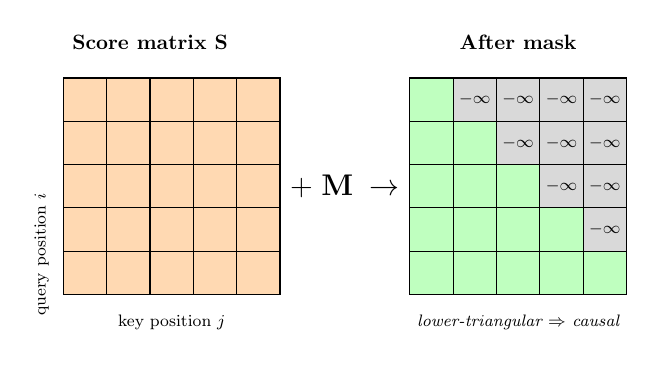
\begin{tikzpicture}[scale=0.55, every node/.style={scale=0.75}]
    % Score matrix (before mask)
    \node[above] at (2,5.5) {\textbf{Score matrix $\mathbf{S}$}};
    \foreach \i in {0,...,4} {
        \foreach \j in {0,...,4} {
            \fill[orange!30] (\j,4-\i) rectangle (\j+1,5-\i);
            \draw (\j,4-\i) rectangle (\j+1,5-\i);
        }
    }
    % Arrow
    \node at (6.5,2.5) {\Large $+\;\mathbf{M}\;\to$};
    % Masked matrix
    \node[above] at (10.5,5.5) {\textbf{After mask}};
    \foreach \i in {0,...,4} {
        \foreach \j in {0,...,4} {
            \pgfmathparse{int(\j<=\i)}
            \ifnum\pgfmathresult=1
                \fill[green!25] (8+\j,4-\i) rectangle (9+\j,5-\i);
                \draw (8+\j,4-\i) rectangle (9+\j,5-\i);
            \else
                \fill[gray!30] (8+\j,4-\i) rectangle (9+\j,5-\i);
                \draw (8+\j,4-\i) rectangle (9+\j,5-\i);
                \node[font=\footnotesize] at (8.5+\j,4.5-\i) {$-\infty$};
            \fi
        }
    }
    % Labels
    \node[below, font=\footnotesize] at (2.5,-0.3) {key position $j$};
    \node[left, font=\footnotesize, rotate=90] at (-0.5,2.5) {query position $i$};
    \node[below, font=\footnotesize\itshape] at (10.5,-0.3) {lower-triangular $\Rightarrow$ causal};
\end{tikzpicture}
\end{document}
